\subsection{Translational Controller}
The movements of the quadcopter along the inertial frame directions x, y and z are controlled by the translational controllers. It is decided to structure the controllers as cascade loops. The relation between the controllers are presented in \autoref{fig:cascade}.

%The translational control systems for x and y are structured as cascade, where the velocity and position are controlled in the inner and outer loop respectively.

\begin{figure}[H]
	\centering
	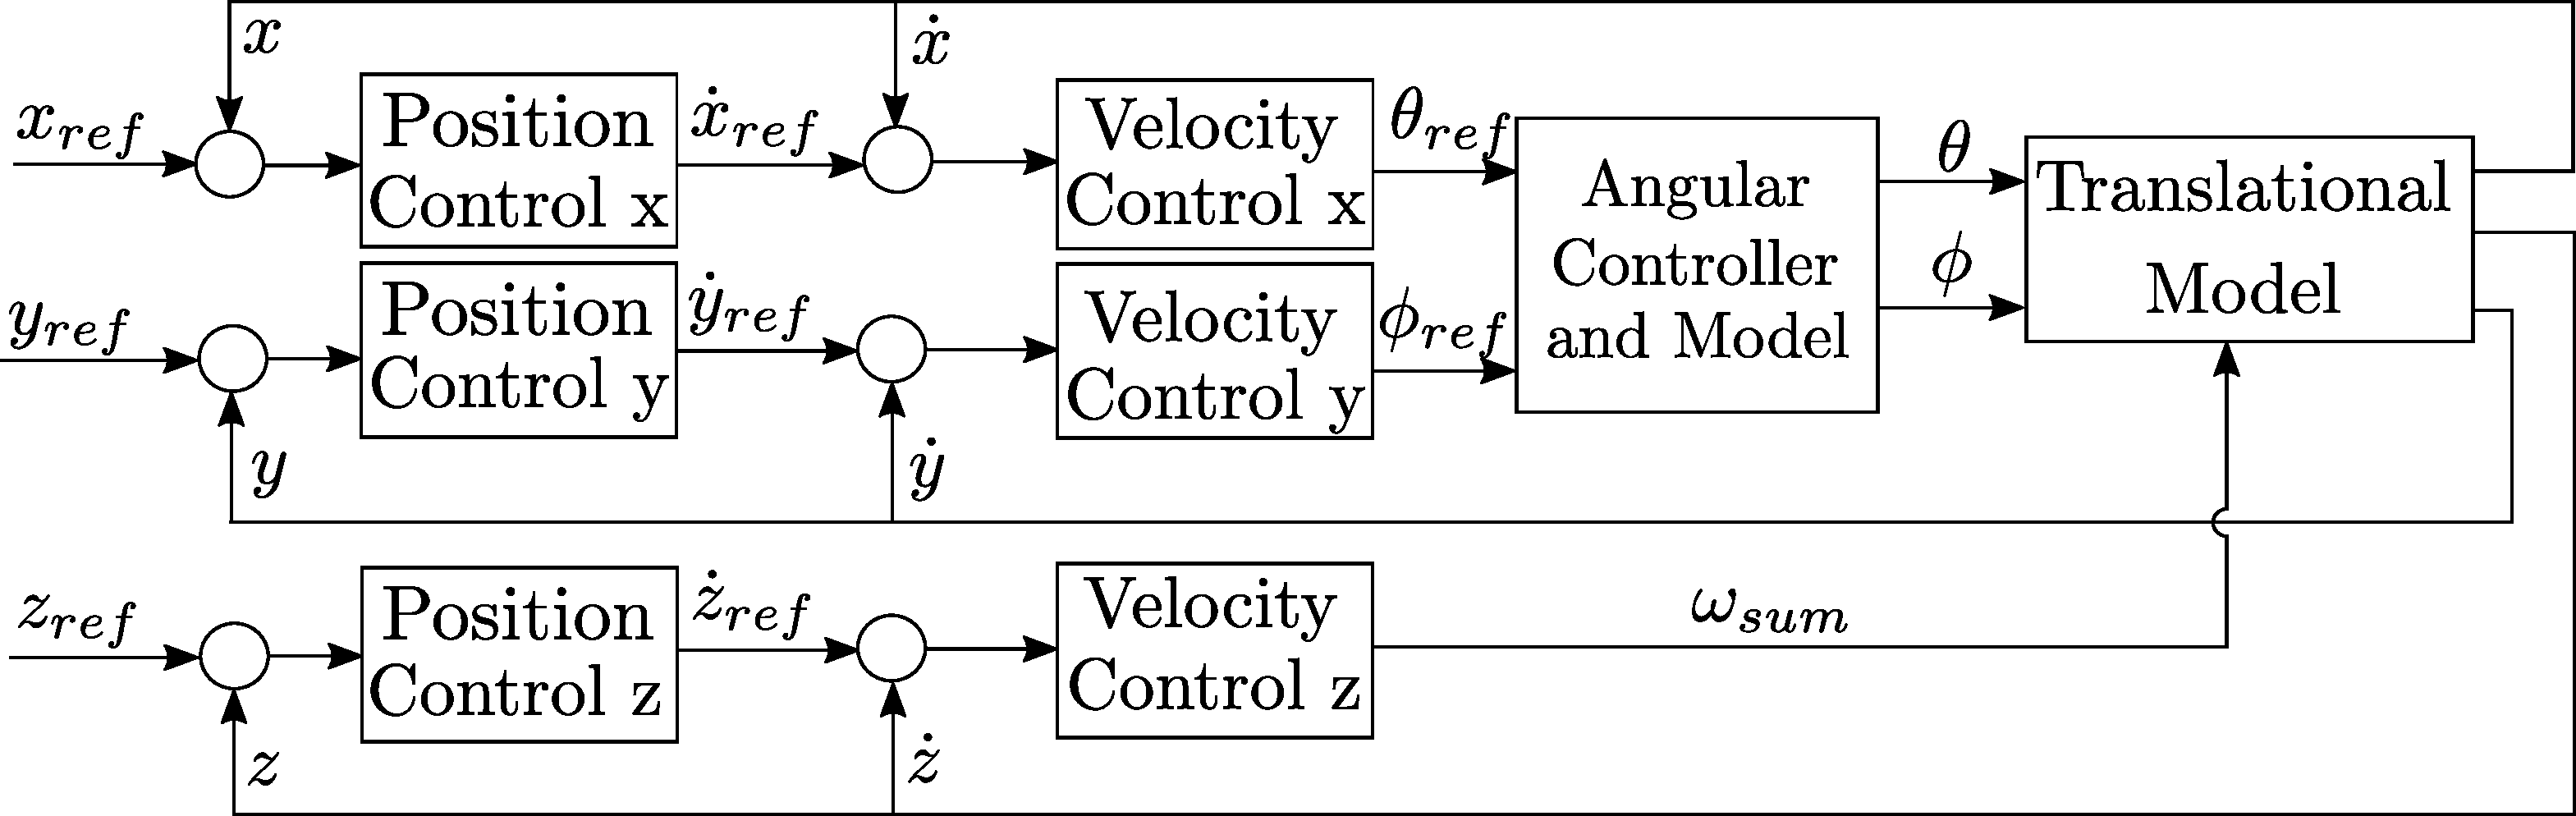
\includegraphics[scale=0.17]{figures/TranslationalControlDiagram.pdf}
	\caption{Overview of control structure.}
	\label{fig:cascade}
\end{figure}
The vertical position is controlled by the cascade loop for the z axis' velocity and position, obtaining the required sum of motor rotational speeds. 
The x and y controller share similar properties as the output for each are an angle reference, namely $\theta_{ref}$ and $\phi_{ref}$ respectively.
Firstly the x and y controllers are designed similarly followed by an individual design for the z controller.\\ 

The inner loop for the x and y translational controllers are now designed followed by the outer loop.
The model equations derived previously, see Equation \ref{eq:AccelerationEqInertial1} and \ref{eq:AccelerationEqInertial2}, are Laplace transformed and put on transfer function in respect to the inner loop, yielding:
\begin{align}
    G_{\dot{x}}(s)&=\frac{\dot{x} (s)}{\theta (s)}=\frac{-k_{th} (\omega_1 ^2 + \omega_2 ^2 + \omega_3 ^2 + \omega_4 ^2)}{m\ s} \\
    G_{\dot{y}}(s)&=\frac{\dot{y} (s)}{\phi (s)}=\frac{k_{th}(\omega_1 ^2 + \omega_2 ^2 + \omega_3 ^2 + \omega_4 ^2)}{m\ s} 
\end{align}
%
%\begin{where}
%\va{G_{x_I}}{is the plant for the translational velocity in $x_I$ direction}{1}
%\va{G_{y_I}}{is the plant for the translational velocity in $y_I$ direction}{1}
%\end{where}
The plants are similar but with different signs. The controller design is carried out for the x translational velocity and applied to the y translational velocity afterwards.\\
A proportional controller is sufficient as the plant already has an integrator, that will eliminate a steady state error and output disturbances. The gain will be the same for both controllers, but must be negative for the x translational controller in order to compensate for its negative plant as this will otherwise be unstable in the closed loop.

%\begin{where}
%    \va{G_{x_I}}{is the plant for the translational position in $x_I$ direction}{1}
%    \va{G_{y_I}}{is the plant for the translational position in $y_I$ direction}{1}
%\end{where}
The gain is designed such that it encounters a bandwidth that is three times lower than the attitude model to ensure minimum effect of disturbances.
The plant of the outer loop is simply an integrator to transform velocity to position. The controller of the outer loop is a proportional controller. The outer loop is designed to have three times less bandwidth than the inner loop to ensure minimization of disturbances to secure a stable system.

The inner loop for the z translational controller is first designed followed by the outer loop.
The model equation derived previously, see Equation \ref{eq:AccelerationEqInertial3} is Laplace transformed and put on transfer function, where the velocity in z direction is the output and the sum of motor rotational speeds is input:
\begin{align}
G_{\dot{z}}=\frac{\dot{Z}}{\omega_{sum}} &= \frac{ \frac{1}{4}\ (-2 k_{th})\ \overline{\omega}_{sum} }{ m\ s } & \label{eq:linearTransferFunctionZ}
\end{align}
Due to an integrator and a negative gain the system's locus will move into the right half plane as the gain increases.
A p controller with negative gain will ensure the locus will move into the left half plane and becoming stable. However, due to input disturbances an integrator is added, as this will eliminate this issue. 
%As the feedback loop now holds two poles in zero, the root locus system will branch along the imaginary axis. A differentiator is added to attract the poles and by that eliminating oscillations.
The final z translational controller of the inner loop is a PI-controller. 

Before the designed controllers can be implemented on the micro controller on the quadcopter, they must be discretized. 
The discretization is done as billinear approximation, also known as Tustin, where the half plane side in Laplace domain is mapped as the unit cycle in the discrete domain. 
%\begin{where}
%  \va{\dot{Z}_I}{is the velocity in the z-direction in the inertial system}{}
%  \va{\omega_{sum}}{is the sum of velocities to be controlled}{}
%  \va{\overline{\omega}_{sum}}{is the sum of rotor velocities in equilibrium}{}
%  \va{k_{th}}{is the thrust constant}{}
%  \va{m}{is the mass of the quadcopter}{}
%\end{where}
